\chapter{Background and Theory}
% This chapter should describe the theoretical background needed to understand
% and solve the problem. For instance, a description of the hardware platform
% or specific components involved in this assignment, definition of concepts
% that are important to understand the solution should be summarized here. Add
% citations to show sources whenever appropriate, LaTeX and bibliography
% managers make this easy.

% TODO: Write an introduction to ptxdist usage


\section{Operating Systems}
An operating system is a special piece of software that provides two important functions in a computer:
\begin{itemize}
  \item Managing the hardware resources.
  \item Providing a useful hardware abstraction layer for application programmers.
\end{itemize}
The core of the operating system is called the \emph{kernel} and runs in a privileged software mode that gives the kernel complete access to all hardware resources. The code running outside the kernel is often referred to as the \emph{user space} or the \emph{userland}, and has only restricted access to hardware. Because of this organization, all hardware-related activities necessary to run the operating system is performed by the kernel, and the user space programs only access hardware through \emph{system calls} in the kernel.\cite{modern-operating-systems}

\subsection{Device Drivers}
To more easily manage hardware devices with different characteristics, the kernel contains \emph{device drivers}. A device driver is a program that manages low-level hardware access to a particular device, providing a clean interface for the rest of the kernel programs.

\subsection{Kernel Modules}
It is sometimes necessary to extend the functionality of the kernel, for instance if new hardware becomes available. While this could be achieved by modifying and rebuilding the kernel, a much more attractive alternative is to use \emph{kernel modules}, small programs that are loaded at runtime and extend the kernel with the needed functionality. Device drivers can be added as kernel modules.

\subsection{Related Terminology}
In addition to the concepts described above, several other terms are used in the context of operating systems:
\begin{itemize}
\item \textsl{Boot Loader:} The bootloader is a small program that runs before the operating system starts, and makes the necessary preparations to start the kernel.
\item \textsl{Linux Root Filesystem:} In Linux, the root filesystem is the filesystem available at the top-level directory. It is denoted with a forward slash, "/".
\end{itemize}



\section{PTXdist}
PTXdist is a build system used to develop userland software for embedded platforms running Linux. It can control most parts of the build process:
\begin{itemize}
  \item Download package sources
  \item Extract package sources and apply patches
  \item Configure packages
  \item Build packages
  \item Create filesystem images
  \item Flash filesystem images to target
\end{itemize}
PTXdist builds the Linux kernel used along with the userland software.

\subsection{Project Setup}
Setting up a PXTdist project consists of the following steps:
\begin{itemize}
  \item Selecting a userland configuration.
  \item Selecting a hardware platform.
  \item Selecting a toolchain.
\end{itemize}
The userland configuration defines what user programs will be built for the target platform apart from the kernel, and the hardware platform defines the target platform of the build. The toolchain selected is the toolchain PTXdist should use when building. As PTXdist looks for toolchains in the /opt folder, selecting a toolchain is not always necessary.

\subsection{Building and Flashing}
After the project has been setup, the kernel and the user programs can be built with one simple command:
\lstset{style=lststyle-terminal}
\begin{lstlisting}
ptxdist go
\end{lstlisting}
This will build several filesystem images for the target platform containing the kernel and all userland programs specified by the userland configuration. PTXdist will automatically find out which packages needs to be built, and download them if necessary.

Finally, the images can then be flashed onto the target platform with the command:
\begin{lstlisting}
ptxdist images
\end{lstlisting}
An illustration of how the PTXdist build process might be for a computer game is shown in figure \ref{fig:ptxdist-build-process}.

\begin{figure}[ht]\label{fig:ptxdist-build-process}
  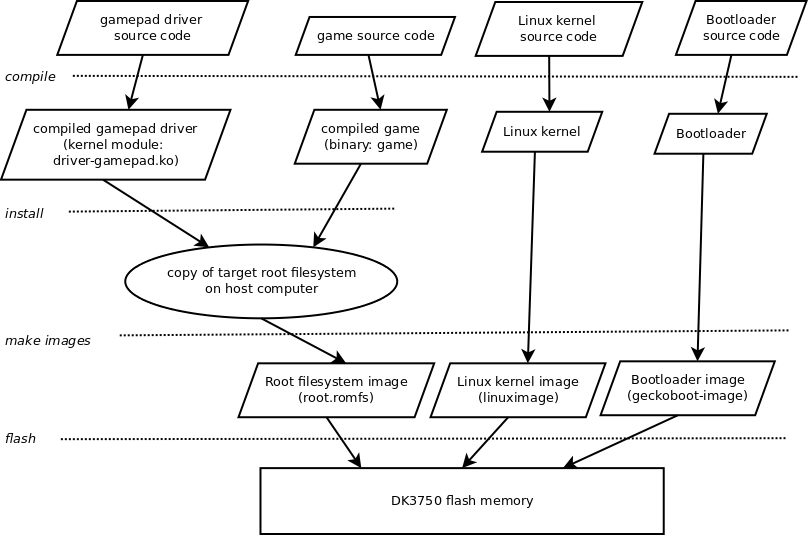
\includegraphics[width=\textwidth]{images/ptxdist_build_process.png}
  \caption{An example overview of a PTXdist build process for a computer game.}
\end{figure}

